\scanpage{18}
\uline{Interprétations en termes de filtrations du foncteur oubli \deleted{sur la catégorie}} des représentations linéaires de dimension finie de $G$. (Il s'agit de filtrations compatibles au produit tensoriel\inserted{%
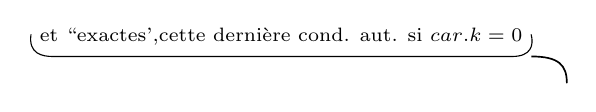
\begin{tikzpicture}[baseline=(tip),x=1cm,y=1cm]
\coordinate (tip) at (6.7,-.48);
\node[anchor=south west,inner sep=0pt,font=\scriptsize] (n) at (0,0) {et ``exactes',cette \unsure{dernière} cond. aut. si $\operatorname{car}.k=0$};
\draw[line width=.4pt] ([xshift=-3pt,yshift=4pt]n.south west) .. controls ([xshift=-4pt,yshift=-3pt]n.south west) and ([xshift=1pt,yshift=-4pt]n.south west) .. ([xshift=5pt,yshift=-4pt]n.south west) -- ([xshift=-4pt,yshift=-4pt]n.south east) .. controls ([xshift=3pt,yshift=-4pt]n.south east) and ([xshift=4pt,yshift=0pt]n.south east) .. ([xshift=3pt,yshift=4pt]n.south east);
\draw[line width=.6pt] (6.25,-.14) .. controls (6.6,-.14) and (6.7,-.25) .. (tip);
\end{tikzpicture}}). Supposons fixé une classe\inserted{%
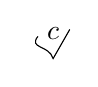
\begin{tikzpicture}[baseline=(tip),x=1em,y=1em]
\coordinate (tip) at (0,0);
\node[inner sep=0pt] at (0,.9) {\handwritten{$c$}};
\draw (-.55,.8) .. controls (-.9,.35) and (-.15,.5) .. (tip) -- (.6,1.05);
\end{tikzpicture}} de\inserted{%
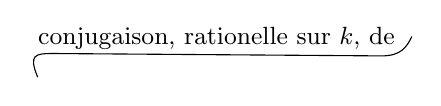
\begin{tikzpicture}[baseline=(tip),x=1cm,y=1cm]
\coordinate (tip) at (0,-.34);
\node[anchor=south west,inner sep=0pt,font=\small] (n) at (0,0) {conjugaison, rationelle sur $k$, de};
\draw (tip) .. controls (-.12,-.05) and (-.03,-.04) .. (.2,-.04) -- ([xshift=-5pt,yshift=-2pt]n.south east) .. controls ([xshift=2pt,yshift=-2pt]n.south east) and ([xshift=4pt,yshift=1pt]n.south east) .. ([xshift=6pt,yshift=5pt]n.south east);
\end{tikzpicture}} telles filtrations (NB elle n'admet pas nécessairement un représentant rat/$k$); i\unsure{%

\begin{tikzpicture}[baseline=(l.base)]
\node[inner sep=0pt] (l) at (0,0) {l};
\node[inner sep=0pt] at (.015em,-.025em) {o};
\end{tikzpicture}}\deleted{\illegible{1}} revient au même de se donner,\deleted{un} pour le Chevalley $G_{\unsure{o|0}}$ associé à $G$, un \deleted{homomorphisme} élément de $\operatorname{Hom}(\underline{G}_m,T_o)/W=M/W$ ($T_o=M\mathbin{\text{\textcircled{x}}}\underline{G}_m$ est le tore maximal type de $G_o$) invariant par le sous-groupe\inserted{%
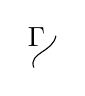
\begin{tikzpicture}[baseline=(tip),x=1em,y=1em]
\coordinate (tip) at (0,0);
\node[inner sep=0pt] at (.1,1.1) {\handwritten{$\Gamma$}};
\draw (tip) .. controls (-.2,.55) and (.7,.55) .. (.8,1.15);
\end{tikzpicture}} de $\operatorname{Auext}G_o=E_o$ image de $\operatorname{Gal}(\handwritten{\bar{k}}/k)$, ou encore un \deleted{homomorphisme $\underline{G}_m\unsure{\to}T$} élément de $M$ qui soit dans la chambre de Weyl de $M\mathbin{\text{\textcircled{x}}}_{\underline{Z}}\underline{R}$ et qui soit stable par $\handwritten{\Gamma}$. On a alors le \unsure{schéma} $\handwritten{\unsure{\underline{\varnothing}|\underline{\phi}}_c}$ des filtrations de classe $\handwritten{c}$, qui est un espace homogène sous $G$, de stabilisateur des points des paraboliques;\inserted{%
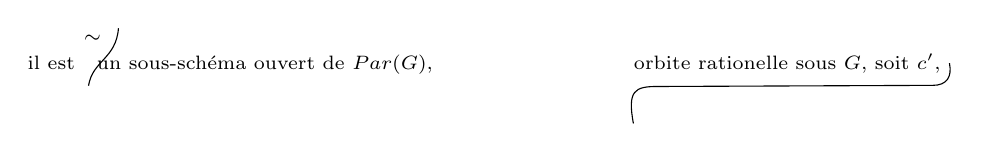
\begin{tikzpicture}[baseline=(tip),x=1cm,y=1cm]
\coordinate (tip) at (7.7,-.5);
\node[anchor=base west,inner sep=0pt,font=\scriptsize] (left) at (0,.18) {\handwritten{il} est\quad un sous-schéma ouvert de $\uline{Par}(G)$,};
\node[inner sep=0pt,font=\scriptsize] at (.83,.58) {\inserted{\handwritten{$\sim$}}};
\draw (.78,-.02) .. controls (.83,.3) and (1.13,.32) .. (1.16,.71);
\node[anchor=base west,inner sep=0pt,font=\scriptsize] (right) at (7.7,.18) {orbite rationelle sous $G$, \handwritten{soit $c'$,}};
\draw (tip) .. controls (7.62,-.08) and (7.72,-.03) .. (8,-.03) -- ([xshift=-3pt,yshift=-4pt]right.south east) .. controls ([xshift=2pt,yshift=-4pt]right.south east) and ([xshift=4pt,yshift=-1pt]right.south east) .. ([xshift=3pt,yshift=4pt]right.south east);
\end{tikzpicture}} On peut regarder aussi le schéma $\operatorname{ST}_c$ des homomorphismes $i:\underline{G}_m\handwritten{\to}G$ de classe $c$, qui est donc une orbite rationelle de $G$ opérant sur $\uline{Homgr}(\underline{G}_m,G)$. Il est canoniquement isomorphe au schéma des couples de Lévi $(P,L)$ tels que $P$ soit de classe $c'$. (En d'autres termes, grâce au choix d'un $c$, pour $P$\inserted{%
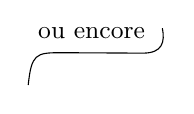
\begin{tikzpicture}[baseline=(tip),x=1cm,y=1cm]
\coordinate (tip) at (0,-.43);
\node[anchor=south west,inner sep=0pt,font=\small] (n) at (.12,.08) {ou encore $\handwritten{\underline{\varnothing}}$};
\draw (tip) .. controls (.04,-.04) and (.1,-.02) .. (.4,-.02) -- ([xshift=-4pt,yshift=-3pt]n.south east) .. controls ([xshift=3pt,yshift=-3pt]n.south east) and ([xshift=4pt,yshift=1pt]n.south east) .. ([xshift=3pt,yshift=6pt]n.south east);
\end{tikzpicture}} de classe $c'$ donné, il revient au même de se donner un $i:\underline{G}_m\handwritten{\to}P$ de la classe définie par $c$, où un sous-groupe de Lévi de $P$, à $i$ étant associé \unsure{\tikz[baseline=-.45ex]{\fill[rotate=-35] (0,0) ellipse (.35pt and .65pt);}} $\operatorname{Cent}(i)$.\handwritten{)} On a %
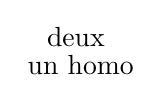
\begin{tikzpicture}[baseline=(old.base),x=1em,y=1em]
\node[anchor=base west,inner sep=0pt] (old) at (0,0) {\deleted{un homo}};
\node[anchor=base west,inner sep=0pt] at (.7,1) {\inserted{deux}};
\end{tikzpicture}morphismesde schémas canoniquement isomorphes
\[
\operatorname{ST}_c\handwritten{\longrightarrow\underline{\varnothing}}_c\quad,\quad
(\operatorname{CL})_{c'}\handwritten{\longrightarrow}\operatorname{Par}_{c'}\quad,
\]
le premier en termes de théorie des filtrations d\unsure{%

\begin{tikzpicture}[baseline=(a.base)]
\node[inner sep=0pt] (a) at (0,0) {a};
\node[inner sep=0pt] at (-.015em,.025em) {e};
\end{tikzpicture}} foncteurs fibres, le deuxième \deleted{d}en termes de groupes paraboliques.
% The overprinted l/o after rat/k and a/e after filtrations retain both contours; their chronology is not assigned.
% After the l/o overlap there is one cancelled covered character; \illegible{1} estimates that remnant, not a missing complete word.
% The oblique spot before Cent(i) is preserved graphically with doubt; the full stop after Cent(i) is definite punctuation.

Supposons maintenant que $k$ soit de car. nulle (j'ignore dans quelle mesure c'est vraiment nécessaire). On peut alors considérer le Schéma $\operatorname{Dyn}_c$ des homomorphismes $f:\operatorname{Sl}(2,k)\handwritten{\longrightarrow}G$ tels que $fi_o$ soit de classe $c$. Supposons-le non vide,\inserted{%
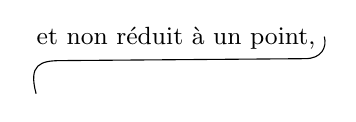
\begin{tikzpicture}[baseline=(tip),x=1cm,y=1cm]
\coordinate (tip) at (0,-.45);
\node[anchor=south west,inner sep=0pt,font=\small] (n) at (0,.1) {\handwritten{et non réduit à un point,}};
\draw (tip) .. controls (-.1,-.08) and (.05,-.03) .. (.32,-.03) -- ([xshift=-4pt,yshift=-3pt]n.south east) .. controls ([xshift=2pt,yshift=-3pt]n.south east) and ([xshift=4pt,yshift=1pt]n.south east) .. ([xshift=3pt,yshift=5pt]n.south east);
\end{tikzpicture}} i.e. $c$ une classe de Dynkin\inserted{%
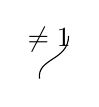
\begin{tikzpicture}[baseline=(tip),x=1em,y=1em]
\coordinate (tip) at (0,0);
\node[inner sep=0pt] at (.35,1.4) {\handwritten{$\ne1$}};
\draw (tip) .. controls (-.1,.75) and (1.05,.65) .. (1.05,1.55);
\end{tikzpicture}}. Alors $\operatorname{Dyn}_c$ est un \deleted{\uline{torseur}}\inserted{\handwritten{espace homogène}} sous $G$\inserted{%
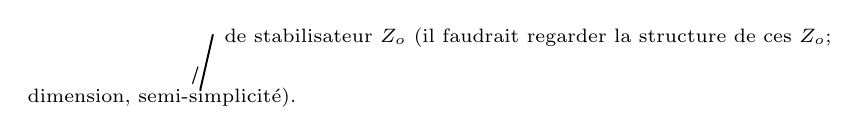
\begin{tikzpicture}[baseline=(tip),x=1cm,y=1cm]
\coordinate (tip) at (2.2,.05);
\node[anchor=base west,inner sep=0pt,font=\scriptsize] at (2.5,.65) {\handwritten{de stabilisateur $Z_o$ (il faudrait regarder la structure de ces $Z_o$;}};
\node[anchor=base west,inner sep=0pt,font=\scriptsize] at (0,-.12) {\handwritten{dimension, semi-simplicité).}};
\draw[line width=.7pt] (2.2,.05) -- (2.36,.75);
\draw[line width=.4pt] (2.1,.12) -- (2.17,.34);
\end{tikzpicture}}\deleted{(en fait, il est can. is. au torseur $\uline{Isom}(G_1,G)$, où $G_1$ est le groupe quasi-déployé correspondant à $G$).} Soit $\operatorname{Un}_c$ le schéma des éléments unipotents\inserted{%
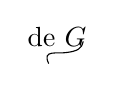
\begin{tikzpicture}[baseline=(tip),x=1em,y=1em]
\coordinate (tip) at (0,0);
\node[inner sep=0pt] at (.3,.95) {\handwritten{de $G$}};
\draw (tip) .. controls (-.25,.52) and (.3,.34) .. (.65,.4) .. controls (1.05,.45) and (1.2,.55) .. (1.25,.8);
\end{tikzpicture}} dont la classe corresponde à \deleted{celle de} $c$ par la correspondance
% archive sheet number: 17
